\documentclass[border=5pt]{standalone}
\usepackage{tikz}
\usepackage{pgfplots}
\pgfplotsset{compat=1.18}

\begin{document}
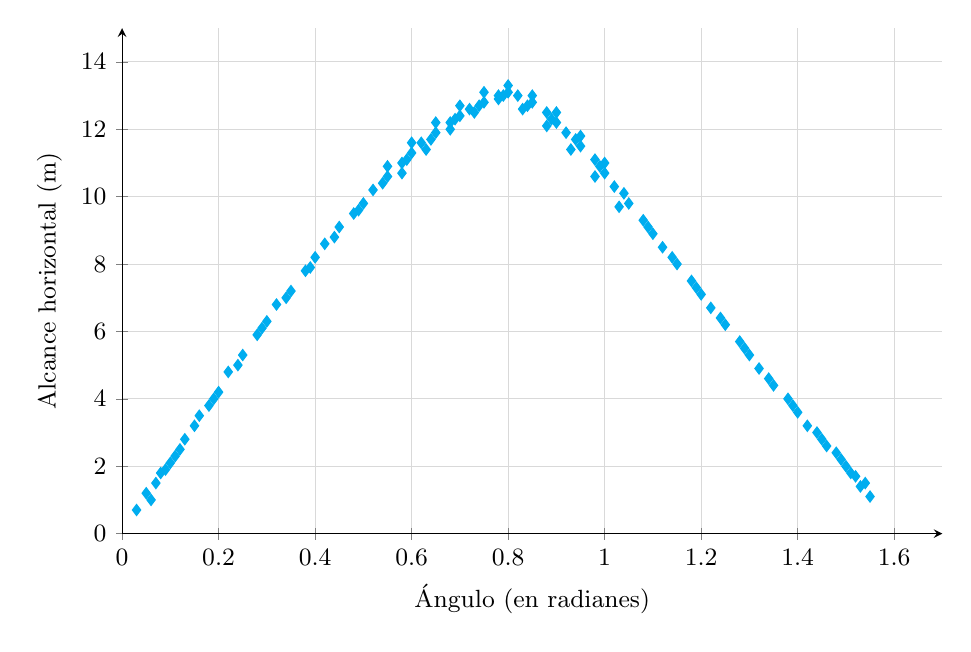
\begin{tikzpicture}
\begin{axis}[
    width=12cm,
    height=8cm,
    xlabel={Ángulo (en radianes)},
    ylabel={Alcance horizontal (m)},
    xmin=0, xmax=1.7,
    ymin=0, ymax=15,
    xtick={0,0.2,0.4,0.6,0.8,1,1.2,1.4,1.6},
    ytick={0,2,4,6,8,10,12,14},
    grid=major,
    grid style={gray!30},
    axis lines=left,
    tick label style={font=\small},
    label style={font=\small},
]

% Datos generados siguiendo R = v0^2 * sin(2*theta) / g con ruido
% v0 = 11.5 m/s, g = 9.8 m/s^2, ruido proporcional a sqrt(alcance)
\addplot[
    only marks,
    mark=diamond*,
    mark size=2pt,
    color=cyan,
    fill=cyan,
] coordinates {
    (0.05, 1.2) (0.08, 1.8) (0.10, 2.1) (0.12, 2.5) (0.15, 3.2)
    (0.18, 3.8) (0.20, 4.2) (0.22, 4.8) (0.25, 5.3) (0.28, 5.9)
    (0.30, 6.3) (0.32, 6.8) (0.35, 7.2) (0.38, 7.8) (0.40, 8.2)
    (0.42, 8.6) (0.45, 9.1) (0.48, 9.5) (0.50, 9.8) (0.52, 10.2)
    (0.55, 10.6) (0.58, 11.0) (0.60, 11.3) (0.62, 11.6) (0.65, 11.9)
    (0.68, 12.2) (0.70, 12.4) (0.72, 12.6) (0.75, 12.8) (0.78, 13.0)
    (0.80, 13.1) (0.82, 13.0) (0.85, 12.8) (0.88, 12.5) (0.90, 12.2)
    (0.92, 11.9) (0.95, 11.5) (0.98, 11.1) (1.00, 10.7) (1.02, 10.3)
    (1.05, 9.8) (1.08, 9.3) (1.10, 8.9) (1.12, 8.5) (1.15, 8.0)
    (1.18, 7.5) (1.20, 7.1) (1.22, 6.7) (1.25, 6.2) (1.28, 5.7)
    (1.30, 5.3) (1.32, 4.9) (1.35, 4.4) (1.38, 4.0) (1.40, 3.6)
    (1.42, 3.2) (1.45, 2.8) (1.48, 2.4) (1.50, 2.0) (1.52, 1.7)
    % Puntos con dispersión adicional (ruido)
    (0.07, 1.5) (0.13, 2.8) (0.19, 4.0) (0.24, 5.0) (0.29, 6.1)
    (0.34, 7.0) (0.39, 7.9) (0.44, 8.8) (0.49, 9.6) (0.54, 10.4)
    (0.59, 11.1) (0.64, 11.7) (0.69, 12.3) (0.74, 12.7) (0.79, 13.0)
    (0.84, 12.7) (0.89, 12.3) (0.94, 11.7) (0.99, 10.9) (1.04, 10.1)
    (1.09, 9.1) (1.14, 8.2) (1.19, 7.3) (1.24, 6.4) (1.29, 5.5)
    (1.34, 4.6) (1.39, 3.8) (1.44, 3.0) (1.49, 2.2) (1.54, 1.5)
    % Más puntos con mayor dispersión en zona central
    (0.55, 10.9) (0.60, 11.6) (0.65, 12.2) (0.70, 12.7) (0.75, 13.1)
    (0.80, 13.3) (0.85, 13.0) (0.90, 12.5) (0.95, 11.8) (1.00, 11.0)
    (0.58, 10.7) (0.63, 11.4) (0.68, 12.0) (0.73, 12.5) (0.78, 12.9)
    (0.83, 12.6) (0.88, 12.1) (0.93, 11.4) (0.98, 10.6) (1.03, 9.7)
    % Puntos dispersos en extremos (menor dispersión)
    (0.06, 1.0) (0.11, 2.3) (0.16, 3.5) (1.46, 2.6) (1.51, 1.8)
    (0.03, 0.7) (0.09, 1.9) (1.53, 1.4) (1.55, 1.1)
};

\end{axis}
\end{tikzpicture}
\end{document}
